% !TEX TS-program = pdflatex
% !TEX encoding = UTF-8 Unicode


% This file is a template using the "beamer" package to create slides for a talk or presentation
% - Giving a talk on some subject.
% - The talk is between 15min and 45min long.
% - Style is ornate.


% MODIFIED by Jonathan Kew, 2008-07-06
% The header comments and encoding in this file were modified for inclusion with TeXworks.
% The content is otherwise unchanged from the original distributed with the beamer package.


\documentclass{beamer}




% Copyright 2004 by Till Tantau <tantau@users.sourceforge.net>.
%
% In principle, this file can be redistributed and/or modified under
% the terms of the GNU Public License, version 2.
%
% However, this file is supposed to be a template to be modified
% for your own needs. For this reason, if you use this file as a
% template and not specifically distribute it as part of a another
% package/program, I grant the extra permission to freely copy and
% modify this file as you see fit and even to delete this copyright
% notice.




\definecolor{colourname}{rgb}{.125,.5,.25}
\usecolortheme[named=colourname]{structure}
\usefonttheme{serif}
\usefonttheme{structureitalicserif}
\mode<presentation>
{
\usetheme{Warsaw}
% or ...


\setbeamercovered{transparent}
% or whatever (possibly just delete it)
}


\usepackage[english]{babel}
% or whatever


\usepackage[utf8]{inputenc}
% or whatever


\usepackage{palatino}
\usepackage[T1]{fontenc}
% Or whatever. Note that the encoding and the font should match. If T1
% does not look nice, try deleting the line with the fontenc.


\usepackage{graphicx}

% Our macros
\newcommand{\hep}{home equity position}
\newcommand{\Hep}{Home equity position}
\newcommand{\HEP}{Home Equity Position}

% Slideshow Metadata
%%%%%%%%%%%%%%%%%%%%%%%%%%%%%%
\title[Progress] % (optional, use only with long paper titles)
{Progress:}


\subtitle
{Preliminary Investigations of \HEP\ Markets } % (optional)


\author[Searle-White, Baron] % (optional, use only with lots of authors)
{E.~Searle-White\inst{1} \and D.~Baron\inst{2}}
% - Use the \inst{?} command only if the authors have different
% affiliation.


\institute % (optional, but mostly needed)
{
\inst{1}%
Mills College
\and
\inst{2}%
Western Washington University
}
% - Use the \inst command only if there are several affiliations.
% - Keep it simple, no one is interested in your street address.


\date[EUR Introduction] % (optional)
{November 7/ BSM Research Project Progress Talks}


\subject{Financial Mathematics}
% This is only inserted into the PDF information catalog. Can be left
% out.






% If you have a file called "university-logo-filename.xxx", where xxx
% is a graphic format that can be processed by latex or pdflatex,
% resp., then you can add a logo as follows:


% \pgfdeclareimage[height=0.5cm]{university-logo}{university-logo-filename}
% \logo{\pgfuseimage{university-logo}}






% Delete this, if you do not want the table of contents to pop up at
% the beginning of each subsection:
\AtBeginSection[]
{
\begin{frame}<beamer>{Outline}
\tableofcontents[currentsection]
\end{frame}
}

\AtBeginSubsection[]
{
\begin{frame}<beamer>{Outline}
\tableofcontents[currentsection,currentsubsection]
\end{frame}
}

% If you wish to uncover everything in a step-wise fashion, uncomment
% the following command:


%\beamerdefaultoverlayspecification{<+->}






\usepackage{parskip}




\begin{document}


\begin{frame}
\titlepage
\end{frame}


\begin{frame}{Outline}
\tableofcontents
% You might wish to add the option [pausesections]
\end{frame}




% Since this a solution template for a generic talk, very little can
% be said about how it should be structured. However, the talk length
% of between 15min and 45min and the theme suggest that you stick to
% the following rules:


% - Exactly two or three sections (other than the summary).
% - At *most* three subsections per section.
% - Talk about 30s to 2min per frame. So there should be between about
% 15 and 30 frames, all told.
%
% - A conference audience is likely to know very little of what you
% are going to talk about. So *simplify*!
% - In a 20min talk, getting the main ideas across is hard
% enough. Leave out details, even if it means being less precise than
% you think necessary.
% - If you omit details that are vital to the proof/implementation,
% just say so once. Everybody will be happy with that.


\section{Introduction}


\begin{frame}{Introduction}
A few weeks ago, we began our research into \hep\ markets. To start, we reviewed some relevant topics in stochastic calculus, financial analysis, and economics.\bigskip

Each week, we reviewed certain literature and also began to build very basic models that incorporated what we were learning, so each week, the models grew more complex.
\end{frame}

\begin{frame}
Reviewed Topics:
\begin{itemize}
\item
Stochastic Calculus
\begin{itemize}
\item 
SDEs
\item
Stochastic Processes and Option Pricing
\end{itemize}
\item
Modern Portfolio Theory
\item 
Prospect Theory
\end{itemize}
\end{frame}

\section{Reviewed Topics}
\subsection{Stochastic Calculus}
\begin{frame}{Stochastic Calculus}{}
 Stochastic Calculus is frequently used to model movements in markets. It relies on the evaluation of \textit{stochastic processes}, which are processes that involve random behavior.\bigskip
\pause

A stochastic (or random) process models the evolution of a system over time. Unlike in deterministic situations, in a stochastic process even if the initial condition is known, there are several directions in which the process can evolve.

\end{frame}

\begin{frame}{Stochastic Process}
Given a probability space $(\Omega, F, P)$ and a measurable space $(S, \Sigma)$, an $S$-valued stochastic process is a collection of $S$-valued random variables on $\Omega$, indexed by $T$ (time). So, a stochastic or random process $X$ is a collection:
$$
\{X_t : t\in T\}
$$
\pause
Note that there are both discrete and continuous stochastic processes.
\end{frame}

\begin{frame}{Brownian Motion}
In particular, we studied a kind of process called a Brownian Motion or a Wiener Process, which is a very specific kind of random walk.\bigskip

One key aspect of a Brownian Motion $W_t$ ($t$ representing time) is the following:
\pause
\begin{itemize} \item[] For $s\leq t$, $(W_{t}-W_{s}) \sim N(0, t-s)$ \end{itemize}
\end{frame}

\begin{frame}
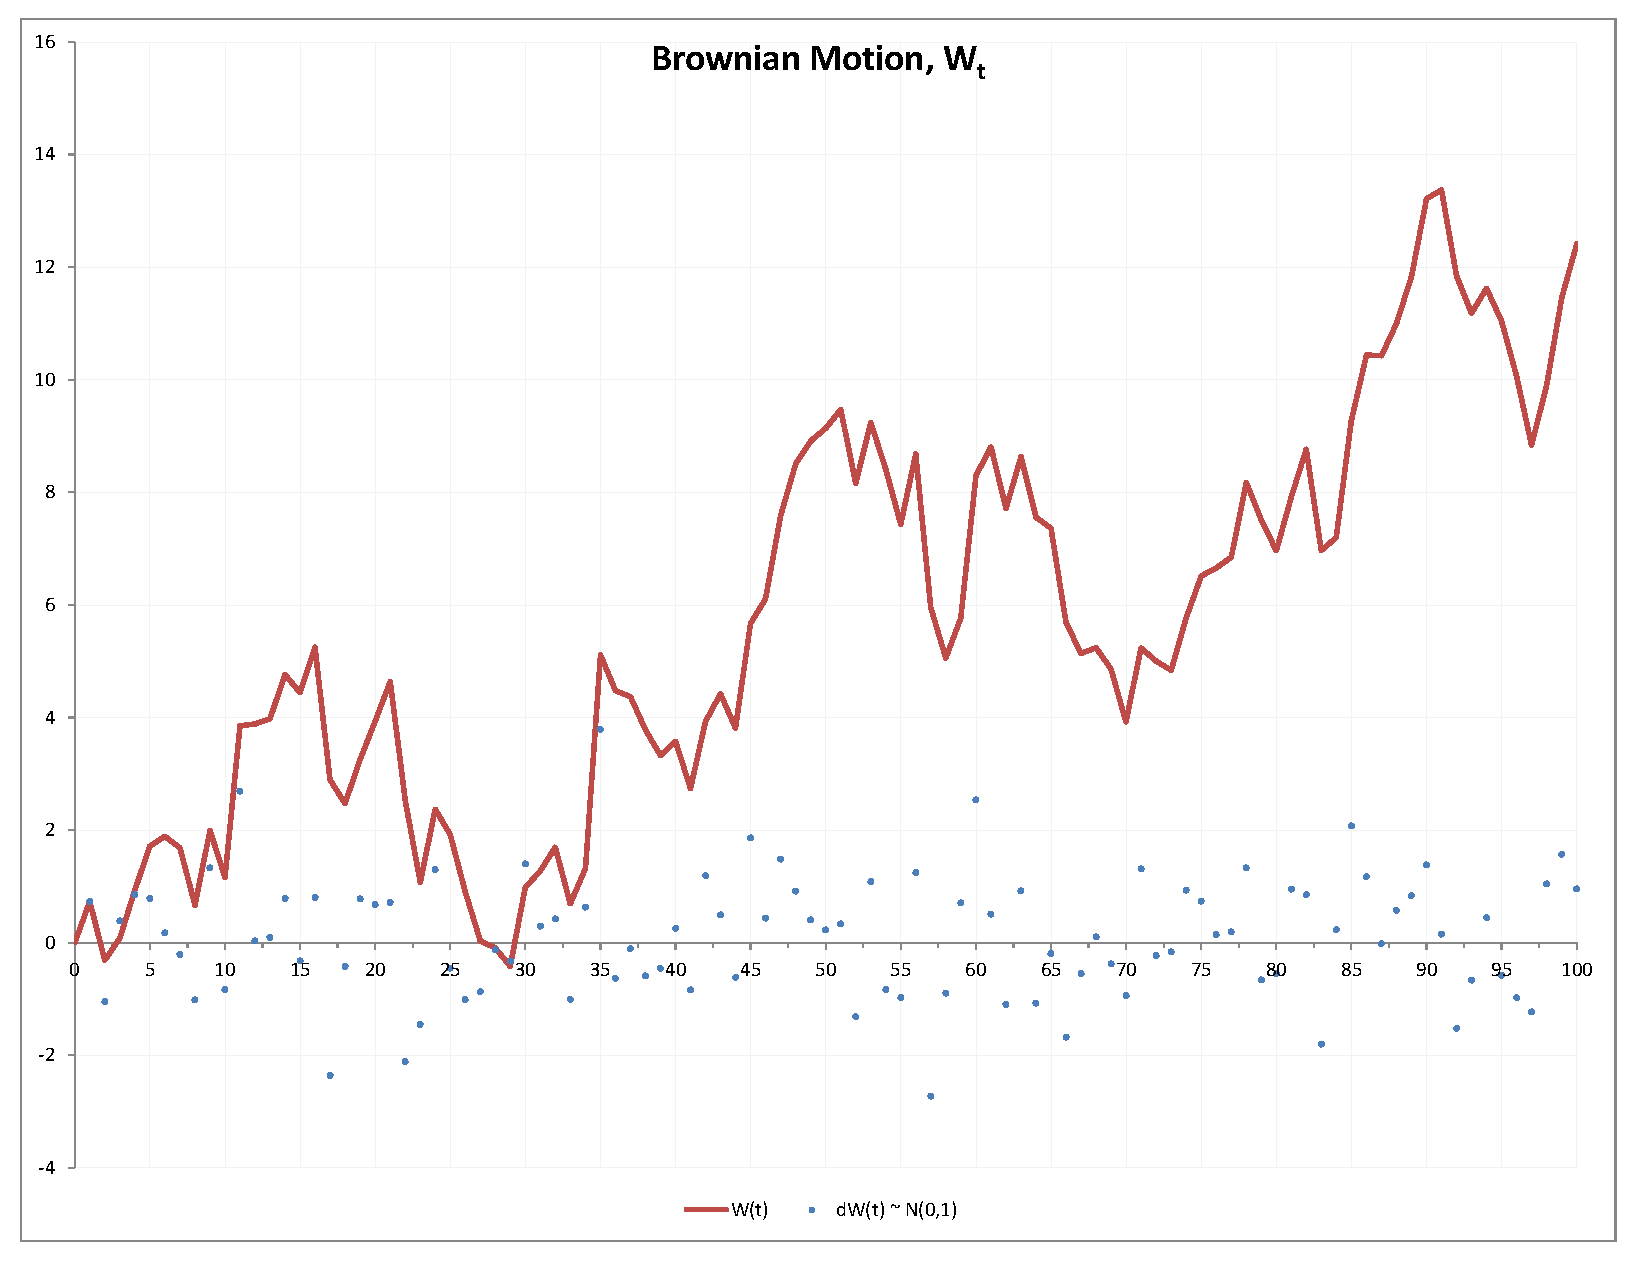
\includegraphics[scale=.35]{brownianchart.pdf}
\end{frame}

\begin{frame}{Stochastic Equations}
 An example of a stochastic process $X_t$, with an underlying Brownian Motion $W_t$, volatility $\sigma$ and drift $\mu$ is:
$$
X_t = X_{0} + \int_0^t\sigma dW_s + \int_0^t\mu ds
$$
\end{frame}

\begin{frame}
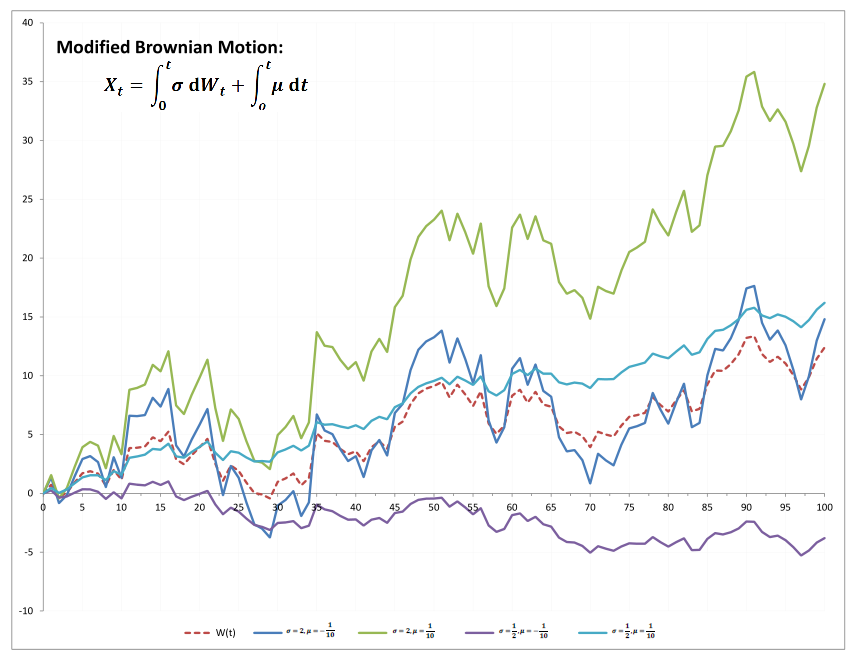
\includegraphics[scale = .45]{sigmaMu.png}
\end{frame}

\begin{frame}{Applications of Stochastic Processes}
\begin{itemize}
\item
One application of such processes is to model home prices over a given time period.
\item
We used the SDE presented before to model logreturns of home prices:
$$
r_t = r_0 + \int_0^t\sigma dW_s + \int_0^t\mu ds
$$
\item
We then applied 
$$
S_t = S_{0}e^{(r_t)}
$$
It is known that the lognormal distribution is very accurate for modeling such prices.
\end{itemize}
\end{frame}

\begin{frame}
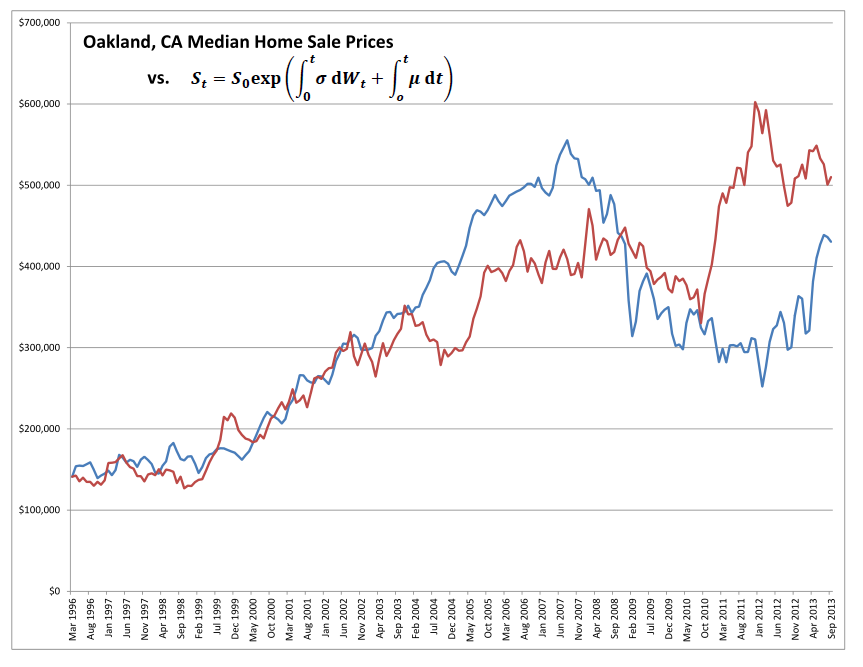
\includegraphics[scale = .45]{lognormal.png}
\end{frame}

\begin{frame}{Applications to the Model}
These and other topics in stochastic calulus helped us to model home appreciation in certain neighborhoods, given that area's volitility, etc. \bigskip

\pause
We used this to track the growth of a home's value in relation to the growth of the neighborhood appreciation in our first model.\\

\end{frame}

\subsection{Portfolio Theory}


\begin{frame}{Portfolio Theory}{Classic and Modern Approaches}
% - A title should summarize the slide in an understandable fashion
% for anyone how does not follow everything on the slide itself.
Portfolio Theory attempts to organize and quantify exactly what the optimal 'portfolio' or bundle of assets for any given investor will be.\bigskip

\pause
In Portfolio Theory, the goal is to correctly structure a group of investments to optimize gain while avoiding risk.
\pause
\begin{itemize}
\item
Correlation
\item
Diversification
\end{itemize}
\end{frame}

\begin{frame}{Portfolio Theory, cont'd}
Tenants of Classic Portfolio Theory:
\begin{itemize}
\pause
\item
Investors are rational and always risk-averse.
\pause
\item
Each investor will tolerate a certain amount of risk in exchange for a return above the \emph{risk-free} return.
\pause
\item
Through these preferences, we can construct a function to determine the optimal portfolio of an investor in terms of risk and return.
\end{itemize}
\end{frame}

\begin{frame}{Indifference Curves}
\includegraphics[scale = .35]{indiff2.png}
\end{frame}

\begin{frame}{Correlation and Diversification}
If $R_p$ is the return of a given portfolio, $R_i$ the return on a specific asset and $w_i$ the weight of asset $i$ (i.e. the proportion of asset $i$ in the portfolio), we have
$$
E(R_p) = \sum_{i} w_i E(R_i)
$$
and the return variance of the portfolio $\sigma_{p}^2$ where
$$
\sigma_{p}^{2} = \sum_{i} w_{i}^{2} \sigma_{i}^{2} + \sum_{i} \sum_{i\neq j} w_{i}w_{j} \sigma_{i} \sigma_{j} \rho_{ij}
$$
Where $\rho_{ij}$ is the correlation coefficient between assets $i$ and $j$.
\end{frame}


\begin{frame}{Applications to the Model}

 Though all \hep s are part of the same market, each individual \hep\ will have its own volatility and trends depending on where the underlying home is located. \bigskip
 
 How do local city economies affect other local economies?
\end{frame}

\subsection{Prospect Theory}
\begin{frame}{Prospect Theory}
The drawbacks of classic portfolio theory are obvious even to an outsider. Prospect theory attempts to uncover and mathematically describe some of the \emph{irrational} behaviors exhibited by investors.\bigskip

\pause
Prospect Theory suggests that when examining a risky prospect, there is an \emph{editing process} investors go through to evaluate the decision at hand.
\end{frame}

\begin{frame}{Anomalies in Decision Making}
\begin{itemize}
\pause
\item
Certainty Effect
\pause
\item
Effect of Small Probabilities
\pause
\item
Framing Effect 
\pause
\item
Isolation Effect

\end{itemize}
\end{frame}


\begin{frame}{Prospect Theory, cont'd}{Applications to the Model}
\pause
Risk assessment by individuals must play a role in our models:
\pause
\begin{itemize}
\item
How do investors evaluate a home before they purchase a \hep ?
\pause
\item
How do investors evaluate potential trades of \hep s?
\pause
\item
How do homebuyers evaluate the outcomes related to selling an equity position in their home?
\end{itemize}
\end{frame}


\section{Model}

\begin{frame}
We have created three simple models thus far.
\pause
\begin{itemize}
\pause
\item
First Model: one neighborhood, one home
\pause
\item
Second Model: three neighborhoods, three homes
\pause
\item
Third Model: three neighborhoods, three homes, one investor
\end{itemize}
\end{frame}


\section{Next Steps}
 \begin{frame}
 To explore:
\begin{itemize}
\pause
\item
When might homeowners sell homes?
\pause
\item
How can we model defaults by homeowners?
\pause
\item
Begin to model the secondary market.
\begin{itemize}
\item
Start with two investors (different preferences), and one home in question.
\end{itemize}
\end{itemize}
\end{frame}

\begin{frame}
\begin{itemize}
\item
How do we model the relationship between investor preferences and home prices?
\item
What kind of bubbles can we expect? How can we accurately model those?
\end{itemize}

\end{frame}

\section{Conclusion}

\begin{frame}
\begin{center}
Questions?
\end{center}
\end{frame}

\begin{frame}
\begin{center}
Thank you for your time and attention.\bigskip

We appreciate the opportunity to pursue this research at BSM.
We are grateful in particular to our project advisors Dezs\H{o} and
Rozi Miklos.
\end{center}
\end{frame}

\begin{frame}
\begin{center}
Reviewed Works
\end{center}
\begin{itemize}
\item
Baxter M. / Rennie A. \emph{Financial Calculus: An Introduction to Derivative Pricing}. Cambridge, UK: Cambridge University Press. 1996.
\item
Hull, J. \emph{Options, Futures, and Other Derivatives}. Upper Saddle River, NJ: Pearson Education, Inc. 2009.
\item
Miklos, R. "Prospect Theory and its Financial Applications". Universiteit van Amsterdam. 2011.
\item
Shreve, S. \emph{Stochastic Calculus for Finance II :Continuous-Time Models}. Pittsburgh, PA: Springer. 2008.
\end{itemize}
\end{frame}

\end{document}






